% PROJECT: <ETD> Electronic Thesis and Dissertation Initiative
%   TITLE: LaTeX report template for ETDs in LaTeX
%  AUTHOR: Neill Kipp, nkipp@vt.edu
%     URL: http://etd.vt.edu/latex/
% SAVE AS: etd.tex
% REVISED: September 6, 1997 [GMc 8/30/10]
% 

% Instructions: Remove the data from this document and replace it with your own,
% keeping the style and formatting information intact.  More instructions
% appear on the Web site listed above.

%\documentclass[12pt,dvips]{report}
\documentclass[12pt]{article}

\setlength{\textwidth}{6.5in}
\setlength{\textheight}{8.5in}
\setlength{\evensidemargin}{0in}
\setlength{\oddsidemargin}{0in}
\setlength{\topmargin}{0in}

\setlength{\parindent}{0pt}
\setlength{\parskip}{0.1in}

% Uncomment for double-spaced document.
% \renewcommand{\baselinestretch}{2}

% \usepackage{epsf}

% BHH Packages
\usepackage[]{mcode}
\usepackage[retainorgcmds]{IEEEtrantools}
\usepackage{amsmath}
\usepackage{amssymb}
\usepackage{graphicx,dblfloatfix}
\usepackage{subfig}
\usepackage{hyperref}
\graphicspath{ {./images/} }
\hypersetup{
    colorlinks=true,
    urlcolor=blue,
    citecolor=black,
    linkcolor=black
}
\usepackage[section]{placeins}
\usepackage{caption}
\setlength{\captionmargin}{20pt}
% END BHH Packages


\begin{document}

\newcommand{\fourier}{\mathcal{F}}
\newcommand{\at}{{\fontfamily{ptm}\selectfont @}}


% TITLE
\thispagestyle{empty}
\pagenumbering{roman}
\begin{center}

{\large Efficient Simultaneous Detection and Isolation of
Many Linearly Modulated Signals}

\vfill

Brian H. Hulette, Amir I. Zaghloul \\
\{hulettbh, amirz\}\at vt.edu \\
Virginia Polytechnic Institute and State University \\
Dept. of Electrical Engineering

\vfill

(ABSTRACT)

\vfill

\end{center}

One common problem in Software-Defined Radio (SDR) systems is that of detecting
and then isolating narrow signals of interest in wideband sampled data. This
involves using some means to detect the frequency of one or more signals of
interest and then tuning, filtering, and decimating them. This problem is
particularly challenging due to the high sample rate of this wideband data, so
efficient algorithms are very desirable. Solutions to this have applications in
many areas, including both Cognitive Radio and Electronic Warfare.

A framework for simultaneously detecting and sub-band tuning multiple signals
is presented, with a focus on finding an efficient means to combine the two
algorithms.  Detection is performed using the Spectral Correlation Density
(SCD) function which exploits the cyclostationary property of digital signals
\cite{Gardner1}.  These detections are then used to direct a configurable
filter bank which will tune, filter, and decimate all of the detected signals.
Two different configurable filter banks are examined: a polyphase
analysis/synthesis filter bank \cite{Harris2} and an overlap-save filter bank
\cite{Borgerding1}.

MATLAB simulations of this framework using both filter banks have been created,
and are used to evaluate their performance. Measures of average runtime for
each filter bank are presented as a proxy for each algorithm's efficiency for
various numbers of signals of interest.

\vfill

\begin{center}
Keywords: Software-Defined Radio, SDR, Cyclostationarity, Spectral Correlation Density, SCD, Detection, Filter Banks
\\
Copyright 2015, Brian H. Hulette
\end{center}

\vfill

% GRANT INFORMATION

%That this work received support from the Southeastern Universities
%Research Association (SURA) ``Monticello Library Project'' is purely
%coincidental.

\pagebreak

% Dedication and Acknowledgments are both optional
% \chapter*{Dedication}
%\chapter*{Acknowledgments}
%First I must acknowledge the work of both Craig Carlson and Ruth Stoehr.
%The core of my testbed for this project is a robust QPSK Transmitter/Receiver
%pair we designed together for an ECE5654 project in the Spring of 2013.
%
%I would also like to thank the members of my committee, particularly Dr.
%Zaghloul, for their patience and support.
%
%Finally, I would like to thank my friends and family, especially my girlfriend
%Meredith, for helping me through this years long process, and letting me use
%``My Masters" as an excuse for nearly anything.

\tableofcontents
\pagebreak

\listoffigures
\pagebreak

%\listoftables
%\pagebreak

\pagenumbering{arabic}
\pagestyle{myheadings}

\section{Introduction}
\label{sec:intro}
\markright{Brian H. Hulette \hfill Section \ref{sec:intro}. Introduction \hfill}

A common problem when designing a Software-Defined Radio (SDR) system is the
problem of detecting and tuning multiple signals of interest. A typical SDR will sample
at a high rate to acquire a large section of the frequency spectrum (referred
to as a wideband acquisition throughout this paper). Then it will attempt to
detect the frequencies within the acquired range that contain signals of
interest, and then tune, filter, decimate, and demodulate those signals. 

Many popular SDR applications perform this detection step with a ``man in the
loop".  A falling raster of the wideband data is presented and the man in the
loop will select the frequency that he would like to process (\cite{WebSDR}
is a web-based implementation of this concept).  A common example of this is to
acquire a wideband slice of the HAM radio spectrum and then select different
frequencies to demodulate new FM push-to-talk signals and listen to them.

This paper investigates a structure that automates this process - but rather
than processing a single analog signal, this framework is intended to process
an arbitrary number of digital signals at once. Detection is performed by
a cyclostationary detector rather than by a man in the loop. This technique
exploits the cyclostationary properties exhibited by most digital signals with
a fixed symbol rate.  Tuning, filtering, and decimating are performed by
a configurable filter bank, so that many signals can be isolated
simultaneously.  

\begin{figure}[h!]
    \begin{center}
    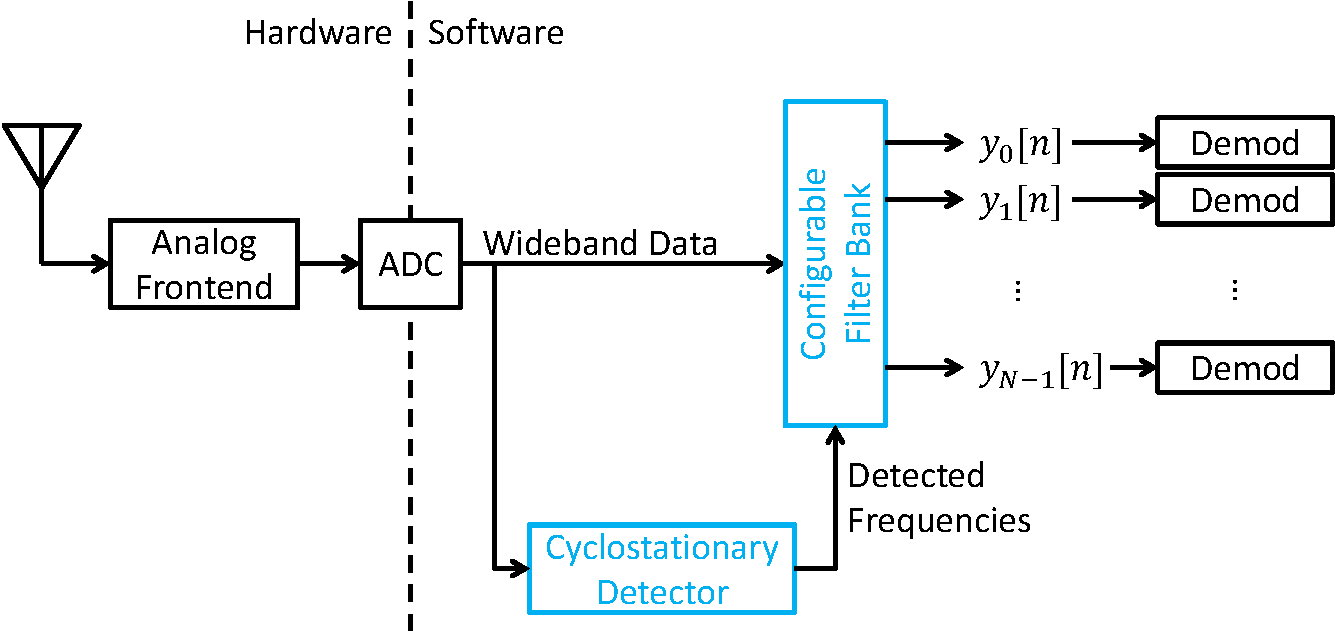
\includegraphics[width=0.8\textwidth]{block_diagram}%
    \end{center}
    \caption{High-level block diagram of our system. An analog front-end and
        ADC are used to bring wideband data into our Software-Defined Radio.
        There, a detector directs a configurable filter bank to isolate $N$
        signals of interest, which are then demodulated. The highlighted
        detector and filter bank are the components examined in this paper.}
    \label{fig:block_diagram}
\end{figure}

The block diagram shown in Figure~\ref{fig:block_diagram} illustrates this
system. A front-end consisting of analog/RF components and an analog-to-digital
converter (ADC) isolate and sample a large section of the frequency spectrum.
This wideband sampled data is then brought into our SDR, where it is processed
by a cyclostationary detector and a configurable filter bank. The frequencies identified by
the detector are fed to the filter bank which will configure itself to isolate
those signals. As the environment changes, with new signals of interest coming
up and current signals going down, the detector will update the filter bank so
it can re-configure itself as needed.

Each of the outputs of the filter bank are sent to a demodulator and/or various
other follow-on processors to extract the signal internals in real-time. These
demodulators must be allocated dynamically as the signal environment changes.

In this paper, we are primarily concerned with two components: the
cyclostationary detector, and the configurable filter bank.  Two different
filter bank structures are examined: an overlap-save filter bank, and
a combined polyphase analysis/synthesis filter bank, composed of a polyphase
analysis filter bank followed by several polyphase synthesis filter banks.
These structures are evaluated on two important criteria:
1) Their ability to accurately reproduce every detected signal, and 2) Their
   computational efficiency when combined with a cyclostationary detector.
% TODO: list papers that discuss SCD for various protocols

Section~\ref{sec:cyclo} provides background information on cyclostationary
properties and the SCD function upon which the detector relies,
Sections~\ref{sec:os_filter_bank} and \ref{sec:poly_chan} describe the
overlap-save filter bank and the polyphase filter bank, respectively. Finally,
Section~\ref{sec:sim} describes the simulation and its results.

\section{Cyclostationary Detection}
\markright{Brian H. Hulette \hfill Section \ref{sec:cyclo}. Cyclotationary Detection \hfill}
\label{sec:cyclo}

\subsection{Cyclostationarity}
\label{sec:cyclo_prop}
Often signals are modeled as stochastic random processes with properties such as
mean and variance, but many man-made signals, particularly digital communications,
can be modeled with another statistical property called
\emph{cyclostationarity}, which implies the signal has some parameter which
varies periodically with time. The frequency of this variation is called the cyclic
frequency, $\alpha$. \cite{Gardner1}.


Of particular interest for this project is second-order cyclostationarity,
where a signal has a periodic auto-correlation, $R_{xx}(t, t+\tau)$:

\begin{IEEEeqnarray}{lCl}
    R_{xx}(t, t+\tau) = E\{x(t)x^*(t+\tau)\} = \sum_{\alpha} R_{xx}^{\alpha}(\tau)e^{j2 \pi \alpha t}
\end{IEEEeqnarray}

The function $R_{xx}^{\alpha}(\tau)$ is the cyclic auto-correlation function (CAF), given by:

\begin{IEEEeqnarray}{lCl}
    R_{xx}^{\alpha}(\tau) = \lim_{T \to \infty} \frac{1}{T}\int_{-T/2}^{T/2} R_{xx}(t, t+\tau)e^{-j2\pi \alpha t} dt
\end{IEEEeqnarray}
The CAF is a function of two parameters, the cyclic frequency, $\alpha$ and the
delay, $\tau$. This function can be used for signal detection in the time
domain. An estimate of the two-dimensional function versus $\alpha$ and $\tau$
is computed, then features within this plane are used for detection (e.g. \cite{Jiandong1, Oner1}).
However, what is of interest for this project is detection in the frequency
domain. This can be performed using the Fourier transform of the CAF, called
the Spectral Correlation Density (SCD), given by:

\begin{IEEEeqnarray}{lCl}
    S_{xx}(\alpha, f) = \int_{-\infty}^{\infty} R_{xx}^{\alpha}(\tau)e^{-j2\pi f \tau} d\tau
\end{IEEEeqnarray}

The SCD is a generalization of the conventional Power-Spectral Density (PSD),
which it reduces to at $\alpha=0$ \cite{Oner1}. Like the CAF, the SCD also
contains unique features based on the modulation type, symbol rate, and carrier
frequency of the transmitted signal(s), which we can exploit for detection.
In \cite{Gardner2}, Gardner defines this SCD for various basic modulation
types, including QPSK, which is used in the presented simulation.

%\section{Exploiting Cyclostationarity for Detection}
%\label{sec:exploit_cyc}
%For the problem defined in Chapter \ref{sec:intro} we can define the wideband
%signal $W(t)$ as the sum of $N$ cyclostationary signals, tuned to
%various frequencies, in an AWGN channel:
%\begin{IEEEeqnarray*}{lCl}
%    W(t) & = & \sum C_{i}(t) e^{j 2 \pi f_i t} + N(t)
%\end{IEEEeqnarray}
%
%Where the $C_i(t)$ are cyclostationary random processes at various symbol rates,
%tuned to corresponding frequencies $f_i$ and $N(t)$ is the AWGN.

%
%We would like to exploit the cyclostationarity of the $C_i$ waveforms to
%identify the frequency, $f_i$, of those waveforms which are transmitted at a
%specific symbol rate.

\subsection{Estimating the SCD}
\label{sec:estimating_scd}
% Use Gardner1 to show that SCD is conjugate multiplication of frequency shifted spectra
% TODO:
% - cyclic wiener relation on Gardner1 pg. 153
% - attempts to derive in lab notebook pg. 20-21
% or just cite Gardner1?
We can estimate a slice of the SCD at cyclic frequency $\alpha$ as
the cross spectral density of the two frequency-shifted time sequences
$x_L(t) = x(t)e^{j\pi\alpha t}$ and $x_U(t) = x(t)e^{-j\pi\alpha t}$ \cite{Gardner1}.

\begin{IEEEeqnarray}{lCl}
    S_{xx}(\alpha, f) & = & X_L(f)X_U^* (f)
\end{IEEEeqnarray}

Note that $x_L(t)$ has been shifted down in frequency by $\alpha/2$, and
$x_U(t)$ has been shifted up by the same amount. In order to estimate the SCD
in this way we must perform two FFTs: one for both $X_L(f)$ and $X_U(f)$.
However, it is possible to estimate both of these spectra using a single FFT,
$X(f)$, in some cases:

\begin{IEEEeqnarray}{lCl}
    S_{xx}(\alpha, f) & = & X_L(f)X_U^* (f) \\
                      & = & X(f - \alpha/2)X^*(f + \alpha/2)
\end{IEEEeqnarray}

Using the second relation we can compute $S_{xx}(\alpha, f)$ using $X(f)$, by
shifting that FFT in either direction by $\alpha/2$, and then conjugate
multiplying the two shifted spectra together. This is significant, since
a simple forward FFT of the acquired data $X(f)$ is useful for other
operations, as we will see in Section~\ref{sec:os_advantages}.

In order to perform this shift accurately using a single FFT we need to
circular shift the FFT by an integer number of bins.  This means we can only
accurately estimate the SCD with this approach when $\alpha/2$ is a multiple of
the FFT resolution.  Thus $\alpha$ must satisfy the following relationship:
\begin{IEEEeqnarray}{lCl}
    \alpha = \frac{2kf_s}{N_{fft}} \text{, } k \in \mathbb{Z}
\end{IEEEeqnarray}
\label{eq:cyclo_freqs}

If an estimate of the SCD at a cyclic frequency that does not satisfy this
relation is required, then we must take the original approach (perform the
frequency shift in the time domain) to be perfectly accurate. Alternatively, we
can still use a single forward FFT and approximate the shift by interpolating
between bins, but this is only an approximation.

\subsection{Using the SCD for Detection}
According to \cite{Gardner2}, QPSK signals generate a large peak in the SCD at
the signal's center frequency when $\alpha$ is equal to the signal baud rate.
So for our application SCD estimates are computed at cyclic frequencies
corresponding to baud rates of interest. Figure \ref{fig:cyclo_estimates} shows
examples of these estimates for our test signal. These plots were generated
using our MATLAB simulation, described in Section~\ref{sec:sim}.

In each of these estimates it easy to detect the large, narrow peak at the
center frequency of the signal with the corresponding baud rate. However, there
are also other features, which agree with the theoretical SCD from
\cite{Gardner2}.  The higher baud rate signals generate wide peaks in the lower
cyclic frequency estimates, like the peak at 2.5 MHz in Figure
\ref{fig:cyclo_156250}. These are easy to distinguish from the main peak with
the human eye since they are much wider, but distinguishing them computationally
is more challenging. The lower baud rate signals also generate features in the
higher cyclic frequency estimates, in the form of two, much smaller peaks,
straddling the actual center frequency. Examples of this are visible around 0 MHz
in Figure \ref{fig:cyclo_312500} and \ref{fig:cyclo_625000}. These features are
easily filtered out by either a human or a computer with a simple threshold.

% TODO: more citations with approaches
There are many potential approaches for identifying signals of interest in
these SCD estimates (e.g. \cite{Thai1,Yoo1}). However, in this paper we are
primarily concerned with efficiently estimating the SCD, so we choose to use
a relatively na{\"i}ve approach: a thresholded peak detection that favors the
higher cyclic frequency SCDs. In the example in
Figure~\ref{fig:cyclo_estimates}, favoring the higher cyclic frequencies allows
us to correctly identify the 625 ksymbol/s signal at
2.5 MHz rather than mistakenly detecting the 156.25 or 312.5 ksymbol/s peaks.

%The second portion of the cyclostationary detection must use these SCD estimates to 
%generate a list of detected frequencies, and the corresponding signal's
%baud rate. In order to do so the following algorithm has been devised. It accepts the input wideband data, and a list of potential baud rates that are of interest.
%
%\begin{enumerate}
%    \item Initialize two empty lists \texttt{f[]} (center frequencies) and \texttt{b[]} (corresponding baud rate for each frequency)
%    \item Sort list of potential baud rates from lowest to highest
%    \item Estimate SCD at $\alpha$ equal to the first (lowest) baud rate
%    \label{loop_ref}
%    \item Detect peaks in the SCD. Use a threshold and a minimum peak separation
%        to filter out false alarms.
%    \item For each detected peak, check if an entry already exists in
%        \texttt{f[]} near that frequency. If so, replace it with this peak's
%        frequency and replace the corresponding entry in \texttt{b[]} with
%        $\alpha$. Otherwise, append a new entry to \texttt{f[]} and
%        \texttt{b[]} with the same values.
%    \item Repeat from \ref{loop_ref} using the next baud rate in the list
%\end{enumerate}
%
%This is a very simple algorithm, but it works well for this test. It is
%fully implemented in the \texttt{cyclostationary\_detect(...)} function. This approach will essentially select the highest symbol rate that appears to be active at a given center frequency.
%
%In an actual application a more robust approach should be used. One possibility
%which could be investigated but is beyond the scope of this project would be to
%use a morphological filter to isolate only very narrow peaks. Between that and
%the thresholding, other features would be easily ignored. For this project the
%simple approach was taken, because the primary focus is on efficiently
%estimating the SCD.

\label{sec:scd_detection}
\begin{figure}[bh!]
\centerline{
    \subfloat[SCD at $\alpha = 0$, Equivalent to a PSD]
    {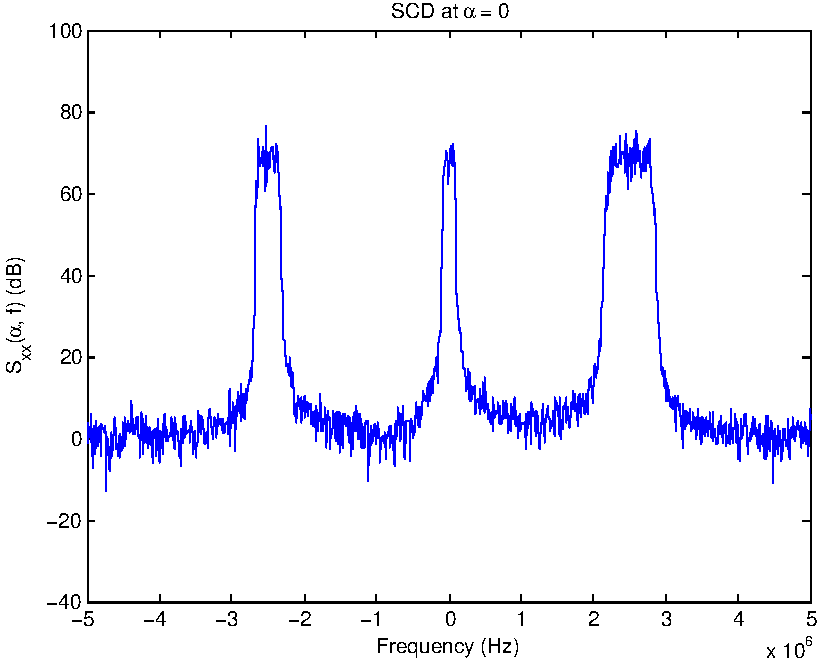
\includegraphics[width=0.45\textwidth]{cyclo_0}%
    \label{fig:cyclo_0}}
    \hfill
    \subfloat[SCD at $\alpha = 156.25$ kHz, baud rate of signal at 0 MHz]
    {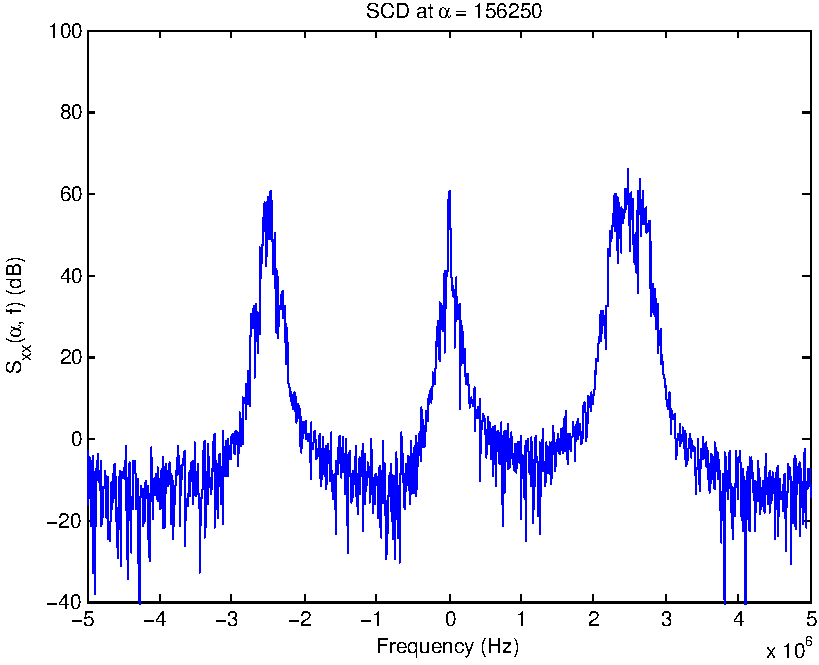
\includegraphics[width=0.45\textwidth]{cyclo_156250}%
    \label{fig:cyclo_156250}}
}
\centerline{
    \subfloat[SCD at $\alpha = 312.5$ kHz, baud rate of signal at -2.5 MHz]
    {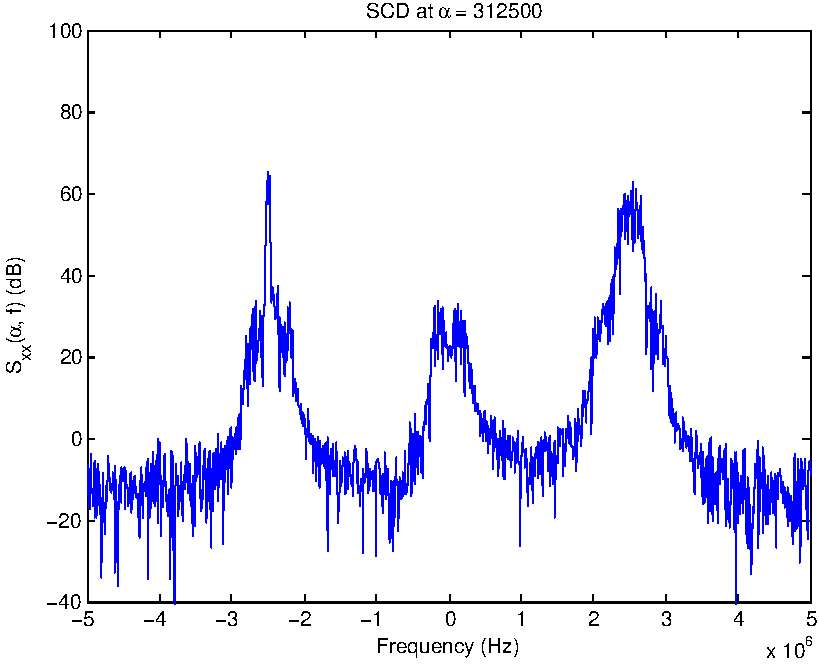
\includegraphics[width=0.45\textwidth]{cyclo_312500}%
    \label{fig:cyclo_312500}}
    \hfill
    \subfloat[SCD at $\alpha = 625$ kHz, baud rate of signal at 2.5 MHz]
    {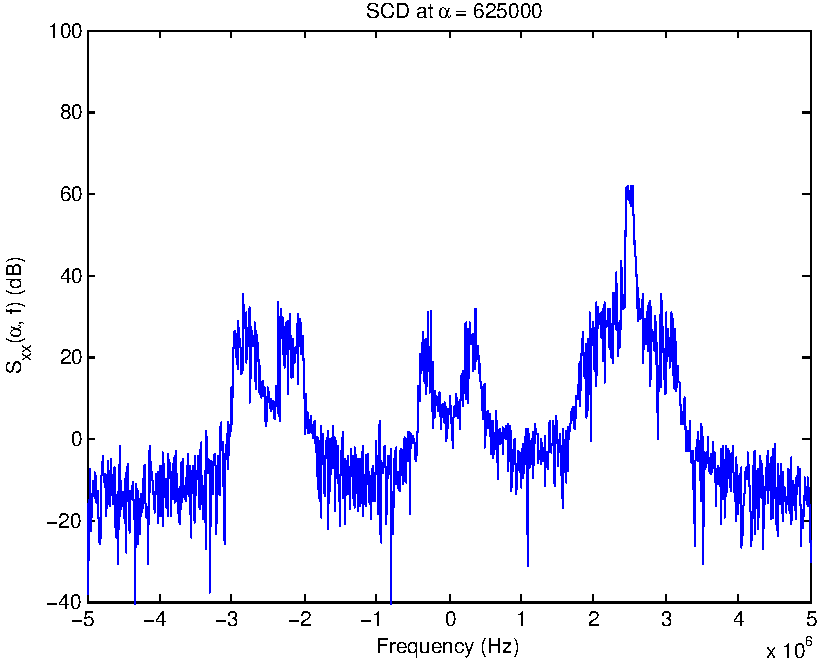
\includegraphics[width=0.45\textwidth]{cyclo_625000}%
    \label{fig:cyclo_625000}}
}
\caption{Estimates of the SCD at various cyclic frequencies for a simulated 
         acquisition with signals at -2.5, 0, and 2.5 MHz.}
\label{fig:cyclo_estimates}
\end{figure}


\section{Overlap-Save Filter Bank}
\markright{Brian H. Hulette \hfill Section \ref{sec:os_filter_bank}. Overlap-Save Filter Bank \hfill}
\label{sec:os_filter_bank}
The overlap-save filter bank structure used in this simulation is based
on a description by Mark Borgerding from March 2006
\cite{Borgerding1}.  Borgerding's concept is based on the well known
Overlap-Save (OS) fast convolution technique.

OS fast convolution can be used to speed up convolution with
a filter that has a long impulse response. The concept is that rather than
convolving in the time-domain, $O(N^2)$, it is faster to first
perform an FFT of both the signal and the filter and conjugate multiply in the
frequency domain, then IFFT to go back to the time domain, $O(N\log_2N)$.
There is nothing new about this idea, but Borgerding's innovation is that he
shows how to extend this concept to tune, filter and decimate any number of
channels with arbitrary center frequencies and bandwidths.

We will now see how the OS filter bank performs tuning, filtering, and
decimation. The same terms that Borgerding defines will be used in this
description:

\begin{center}
\begin{tabular}{ll}
    $x(n)$        & Input data \\
    $h(n)$        & Baseband filter response \\
    $y(n)$        & Tuned, filtered and decimated output data \\
    $P$           & Length of $h(n)$ \\
    $N$           & FFT size \\
    $D$           & Decimation factor \\
    $V = N/(P-1)$ & Ratio of FFT size to filter order \\
\end{tabular}
\end{center}

\emph{Tuning:} If the frequency of the signal of interest corresponds exactly
to one of the FFT bins then we can simply circular shift the FFT output to
place that bin at the center. Then filtering can be performed at baseband.  If
all channels satisfy this criterion then we can re-use a single forward FFT for
every channel, simply by circular shifting it to the appropriate bin in every
case.  This approach is shown in Figure \ref{fig:overlap_save_freq_domain}.

However, if this condition is not satisfied then we will need to perform the
frequency shift in the time domain by multiplying by a complex rotator.
Fortunately, there is a still a way to re-use the forward FFT in this case.
After taking an FFT of the non frequency-shifted signal we can shift the
baseband filter response to the desired center frequency, then after the
filtered signal is returned to the time domain with an IFFT, we perform the
frequency shift with a complex rotator.  In addition to allowing us to re-use
the forward FFT for each channel, this is more efficient than frequency
shifting before the forward FFT since the multiplication is performed after
decimation. This approach is shown in Figure
\ref{fig:overlap_save_time_domain}.

\begin{figure}[bh!]
\centerline{
    \subfloat[Performing frequency shift by circular shifting the FFT output]
    {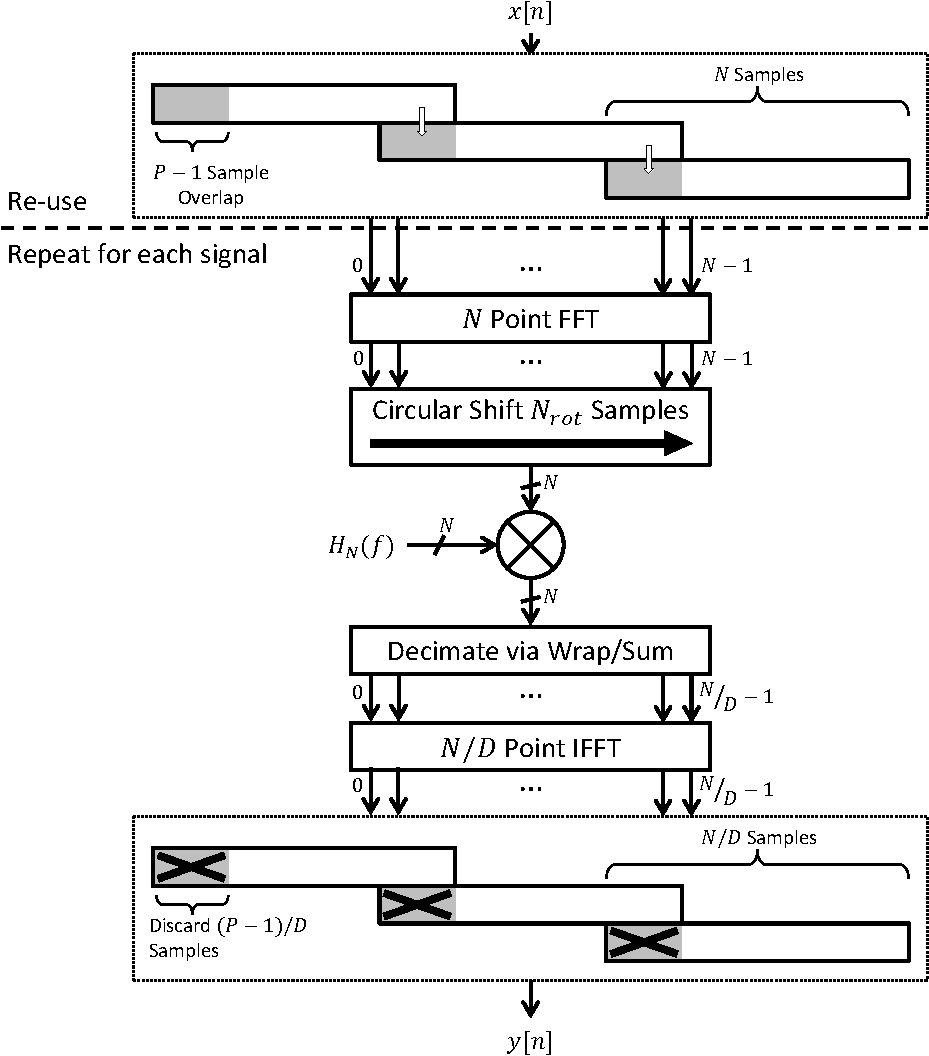
\includegraphics[width=0.48\textwidth]{overlap_save_freq_domain}%
    \label{fig:overlap_save_freq_domain}}
    \hfill
    \subfloat[Performing precise frequency shift in the time-domain]
    {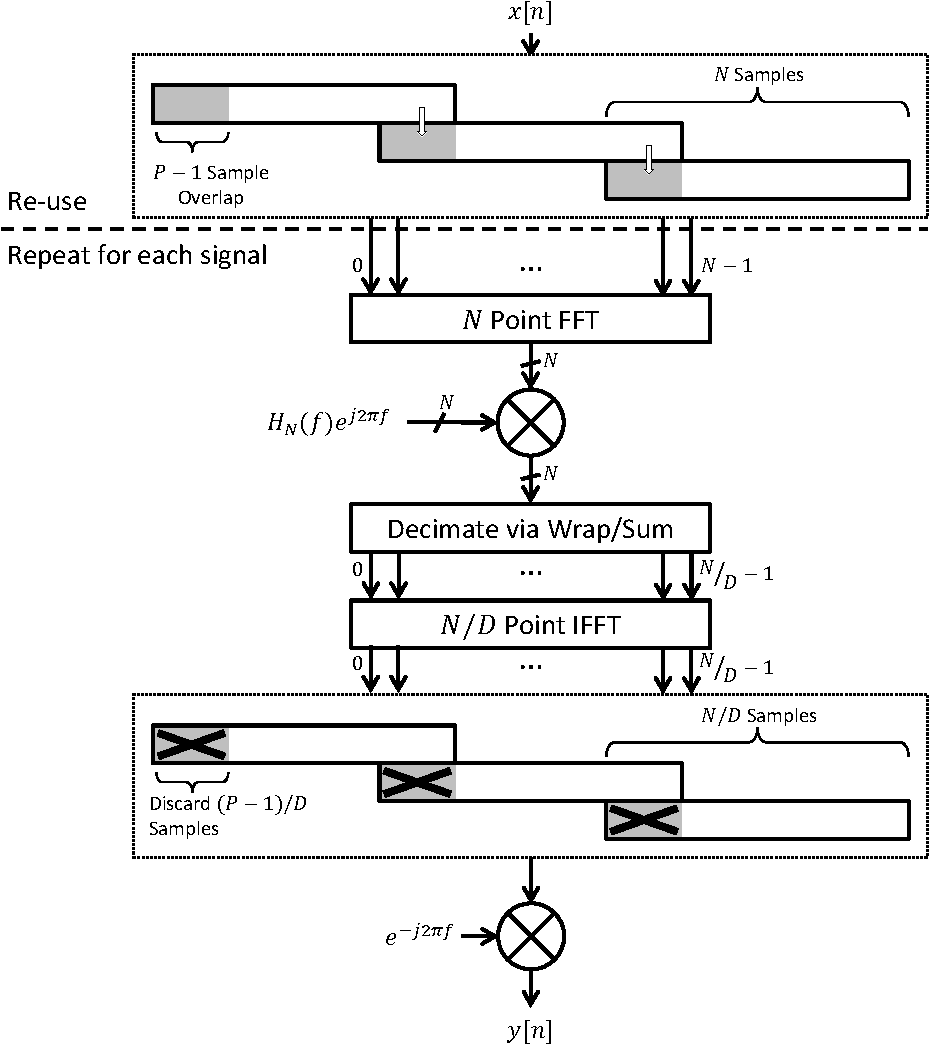
\includegraphics[width=0.48\textwidth]{overlap_save_time_domain}%
    \label{fig:overlap_save_time_domain}}
}
\caption{Overlap-save filter bank structures}
\label{fig:overlap_save_filter_banks}
\end{figure}

\emph{Filtering:} As discussed earlier, this structure relies on OS fast
convolution for filtering. The low-pass filter impulse response for each
channel is Fourier transformed and then conjugate multiplied with the FFT of
the input data after the signal of interest has been tuned to baseband.
Alternatively, if tuning is being performed in the time domain, the filter
impulse response must be tuned up to the signal frequency before being Fourier
transformed.

\emph{Decimation:} Following the frequency domain filtering we have two
different options for decimation. The first option is to perform a full size
inverse FFT of the output, and then decimate in the time domain. The issue with
this approach is that we are computing a larger inverse FFT than we really need
to. Borgerding suggests decimating in the frequency domain as a solution to this.
The approach (called ``Wrap/Sum" in Figure
\ref{fig:overlap_save_filter_banks}) is simple: coherently add together the
components of the frequency spectrum that would be aliased upon time domain
decimation. For example, if the FFT size is 1024 and we need to decimate by
a factor of 4, then coherently sum FFT samples 0 to 255, 256 to 511, 512 to 
767 and 768 to 1024.  The result is a 256 sample frequency
spectrum which we can now inverse FFT to produce the decimated output. The
only trick with this approach is that we must discard just $(P-1)/D$
samples rather than $P-1$ to account for the overlap.  This reveals one
restriction of this structure: the filter order $P-1$ must be an integer
multiple of the decimation, $D$.

\subsection{Limitations}
\label{sec:os_limitations}
There are a few limitations of this structure that are worth mentioning. First,
as mentioned earlier, the filter order $P-1$ must be an integer multiple of the
decimation factor $D$. This problem is pretty easy to solve though - simply
zero-pad the filter to achieve an appropriate length. Another limitation that
is potentially challenging is that the FFT size, $N$, must be an integer
multiple of the decimation rate, $D$. So decimation rates whose prime factors
are larger than 2 or 5 (or others, depending on the FFT implementation) could
lead to FFT inefficiency for this structure.

One more limitation arises when attempting to tune by rotating the FFT, as in
Figure~\ref{fig:overlap_save_freq_domain}.  As previously mentioned, the
precision of the frequency shift is limited by the resolution of the FFT.
However, the precision is also limited further by $V$, the ratio of FFT size to
filter order. This is because we must restrict mixing to the frequencies whose
period completes in $L=N-(P-1)$ samples. Borgerding provides the following
equation for computing the number of FFT bins to rotate to shift to frequency
$f$ (\cite{Borgerding1} Equation (1)):

\begin{equation}
    N_{rot} = \text{round}\left( \frac{Nf}{Vf_s} \right) V
\end{equation}

Where $f_s$ is the wideband sample rate. This equation simply adjusts $N_{rot}$
to the nearest multiple of $V$ bins. It is worth noting that the solution
presented for making $P-1$ an integer multiple of $D$ is only making this
problem worse by making $V$ larger - but there's nothing to be done about that
other than opting for a shorter filter.

The easiest solution to this issue is to simply use the time-domain tuning
approach illustrated in Figure~\ref{fig:overlap_save_time_domain}. It is
slightly more complicated since a new band-pass filter must be generated from
a low-pass prototype for each signal, and a complex rotator is required at the
output, but it can easily select arbitrary frequencies.

\subsection{Advantages}
\label{sec:os_advantages}

The greatest benefit of the overlap-save filter bank for our application is the
ease with which it can be combined with SCD Estimation for cyclostationary
detection. Since the first step for both algorithms is a forward FFT of the
wideband input, when designing a joint cyclostationary detector/overlap-save
filter bank we can re-use the same forward FFT for both algorithms.

% TODO: Image of this combination

The only design challenge is finding a combination of FFT size, sample rate,
and decimation factor that will work for both algorithms.

% TODO: Analysis of this problem. Decimation factor is related to alpha by the amount of oversampling.
% Started this analysis a bit in lab notebook pg. 23

%We can say that the output sample rate is some integer multiple of the symbol rate:
%\begin{equation}
%    f_s' = \beta \alpha \text{, } \beta = 1,2,\hdots
%\end{equation}
%Where the integer multiple $\beta$ is simply the amount of oversampling. Then we can 

Additionally, averaging the overlapped FFT frames together may have an effect
on the accuracy of the SCD estimation, but analyzing this effect is beyond the
scope of this paper.


\section{Polyphase Analysis/Synthesis Filter Bank}
\markright{Brian H. Hulette \hfill Section \ref{sec:poly_chan}. Polyphase Analysis/Synthesis Filter Banks \hfill}
\label{sec:poly_chan}
The second filter bank structure we will examine relies on the analysis and
synthesis polyphase filter banks described by fred harris\cite{Harris1}.
A polyphase analysis filter bank (AFB) can be used to break up a wideband signal into
$M$ distinct channels, each decimated by a factor of $D$ from the wideband
sample rate.  While a polyphase synthesis filter bank (SFB) performs the reverse
operation, combining $M$ channels into one wideband signal. The channel
frequencies used in both structures are given by the expression:

\begin{IEEEeqnarray}{lCl}
    f_k = k \frac{f_s}{M}
\end{IEEEeqnarray}

where $f_k$ is the center frequency of channel $k$ and $f_s$ is the input sample
rate. 

These two structures can be combined to create a very flexible filter bank that
can isolate signals with arbitrary center frequencies and various bandwidths
\cite{Harris2}.

To introduce the concept of analysis and synthesis filter banks we will start
with the maximally-decimated case, where the number of channels, $M$, is equal
to the decimation factor $D$. In \cite{Harris1}, harris shows how the polyphase
AFB works by starting with a basic filter/decimator and making incremental
modifications until it becomes an analysis filter bank as shown in Figure
\ref{fig:polyphase_analysis}. A brief summary of this explanation is provided
here, which follows Figure~\ref{fig:polyphase_proof}.

\begin{figure}[h!]
\centerline{
    \subfloat[Single channel of a simple tuning, filtering, and decimating filter bank. $h(n)$ is a baseband low-pass filter.]
    {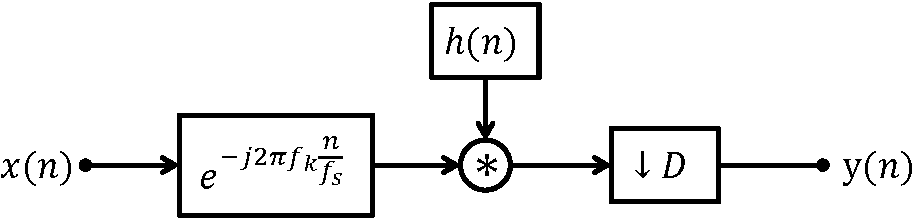
\includegraphics[width=0.45\textwidth]{polyphase_1}%
    \label{fig:polyphase_1}}
    \hfill
    \subfloat[Equivalency theorem allows the tuning step to be moved after the decimation. The baseband filter must be shifted up to $f_k$. If $f_k$ is a multiple of the output sample rate,  $\frac{f_s}{D}$, the tuning step can be dropped.]
    {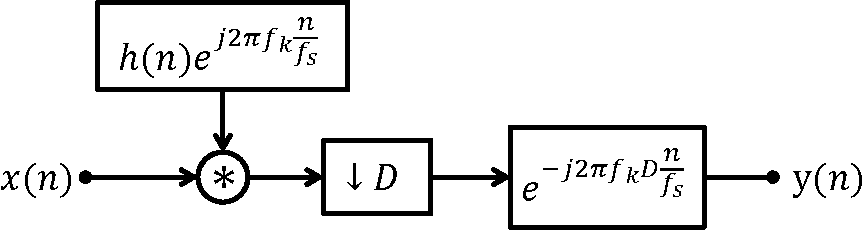
\includegraphics[width=0.45\textwidth]{polyphase_2}%
    \label{fig:polyphase_2}}
}
\centerline{
    \subfloat[The Noble Identity allows the filtering and decimation to be combined to remove excess computations.]
    {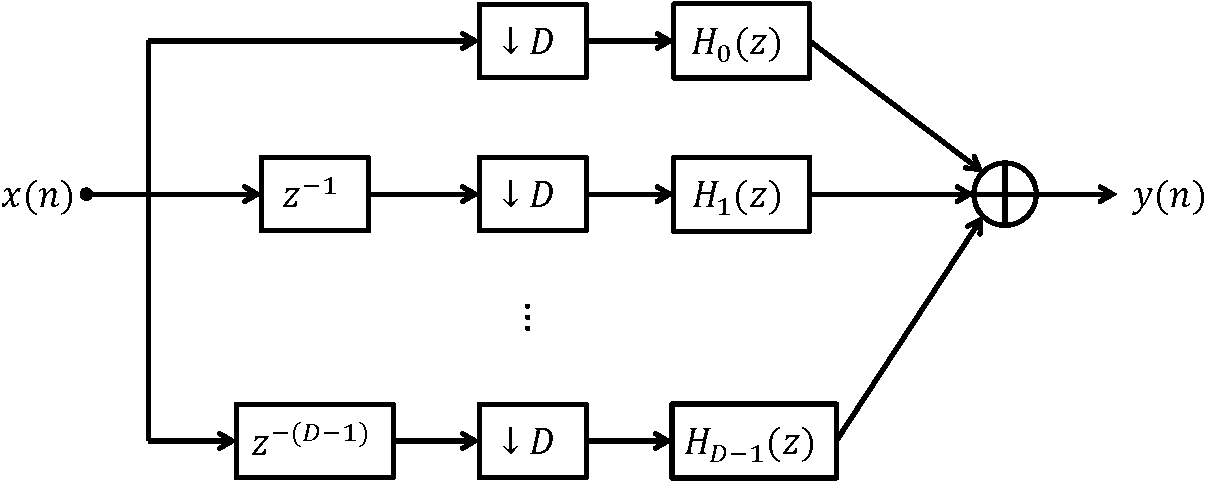
\includegraphics[width=0.45\textwidth]{polyphase_3}%
    \label{fig:polyphase_3}}
    \hfill
    \subfloat[The series of delays and decimation steps can be replaced with an input commutator and complex rotators can be added after each filter to select channel $k$.]
    {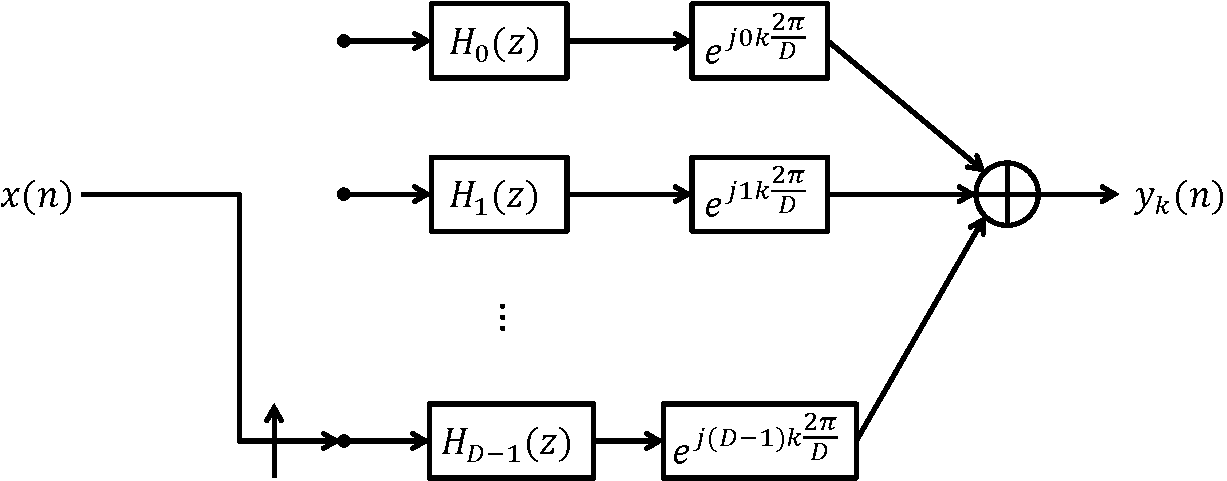
\includegraphics[width=0.45\textwidth]{polyphase_4}%
    \label{fig:polyphase_4}}
}
\caption{Creating a single channel of a polyphase analysis filter bank}
\label{fig:polyphase_proof}
\end{figure}

We start with a single channel of a basic filter bank in Figure
\ref{fig:polyphase_1}. This channel consists of a multiplication with a complex
rotator to tune the desired center frequency down to baseband, followed by
a low-pass filter, represented by $h(n)$, and finally a decimation by $D$. The
first modification we can make takes advantage of the Equivalency Theorem,
which says that we can switch the order of the tuner and the filter, \textbf{if}
the filter is changed to a bandpass filter centered at $f_k$. This modification
is shown in Figure \ref{fig:polyphase_2}. In this figure the tuner has also
been moved after the decimator. Note that if the channel frequency, $f_k$, is
an integer multiple of the output sample rate, $\frac{f_s}{D}$, then the tuner
simplifies to $e^{j2\pi n} = 1$, so it can be dropped completely.  Thus we will
restrict the polyphase analysis filter bank to center frequencies which are
integer multiples of the output sample rate.

Next we can use the Noble Identity to swap the decimator and the filter, as
shown in Figure \ref{fig:polyphase_3}. In order to do so we need to define
a set of partitions of the low-pass filter, $H_r(z)$, such that:

\begin{IEEEeqnarray}{lCl}
    H(z) = H_0(z^D) + z^{-1}H_1(z^D) + \hdots + z^{-(D-1)}H_{D-1}(z^D)
\end{IEEEeqnarray}

This means that each filter, $H_r(z)$, has has an impulse response which is
$h(n)$ shifted by $r$ samples and decimated by $D$. Using the Noble Identity in
this way saves us from computing samples that will just be dropped by the
decimator. Note that in Figure \ref{fig:polyphase_3} the tuner has been dropped
as well, since we are restricting the filter bank to frequencies which are
multiples of the output sample rate.

Finally, we complete the structure for a single channel of a polyphase analysis
filter bank in Figure \ref{fig:polyphase_4}. The combination of delays and
decimators at the front of the previous structure is actually just
a commutator. In \cite{Harris1} Harris explains this by thinking about the
decimators as a switch that closes every $D$ samples. So in Figure
\ref{fig:polyphase_3}, when all of the switches close the filter at the bottom
gets the oldest sample, and each filter as you go up gets one newer sample
until you get to the most recent sample on the top. The next sample is not
processed until the switches close again, and it is passed to the filter at the
bottom. With this explanation it is easy to see the whole structure can be
replaced with a commutator.

The final structure has one more modification. The outputs are multiplied by
complex rotators which select the individual channel, $k$, centered at $f_k$.
A detailed explanation of this can be found in \cite{Harris1}. When all of the
channels are combined to form the full filter bank these complex rotators all
represent a DFT.  The set of rotators that are multiplied and then summed
together for channel $k$ correspond to the $k$th output of a DFT:

\begin{IEEEeqnarray}{lCl}
    y_k(n) & = & \sum_{r=0}^{D-1} y_r(n) e^{j(2\pi/D)rk} 
\end{IEEEeqnarray}

Where $y_r(n)$ represents the output of filter $H_r(z)$, and $y_k(n)$ is the
output of channel $k$. Thus we can compute all $D$ of the complex rotators with
a $D$ point FFT, as shown in Figure \ref{fig:polyphase_analysis}. 

Figure \ref{fig:polyphase_synthesis} shows the complementary structure: the
polyphase synthesis filter bank. It is essentially a mirror image of the
analysis case - an IFFT followed by filters and a commutator. It combines $M$
channels at an equal sample rate, $f_s$, into a single wideband signal at
sample rate $Mf_s$.  The following section shows how these two structures can
be used together to produce a very flexible filter bank.

\begin{figure}[h!]
\centerline{
    \subfloat[Analysis]
    {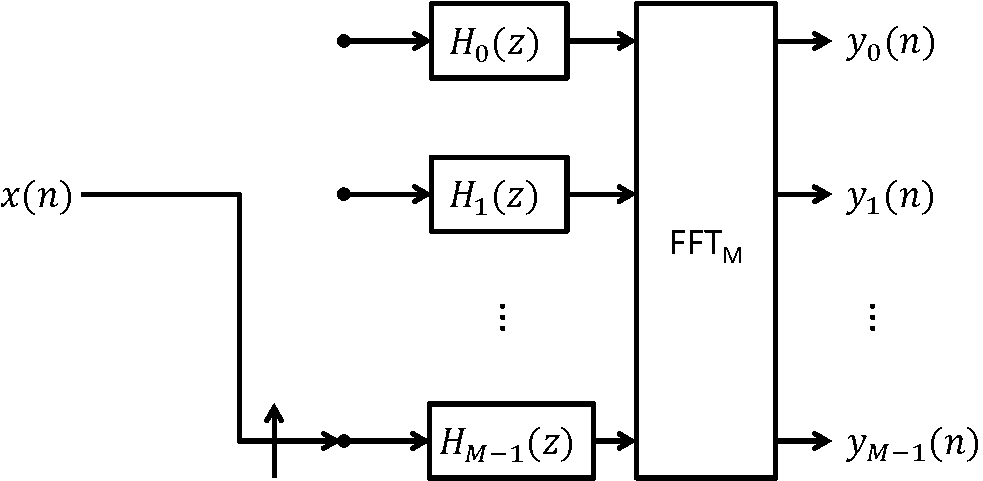
\includegraphics[height=4cm]{polyphase_analysis}%
    \label{fig:polyphase_analysis}}
    \hfill
    \subfloat[Synthesis]
    {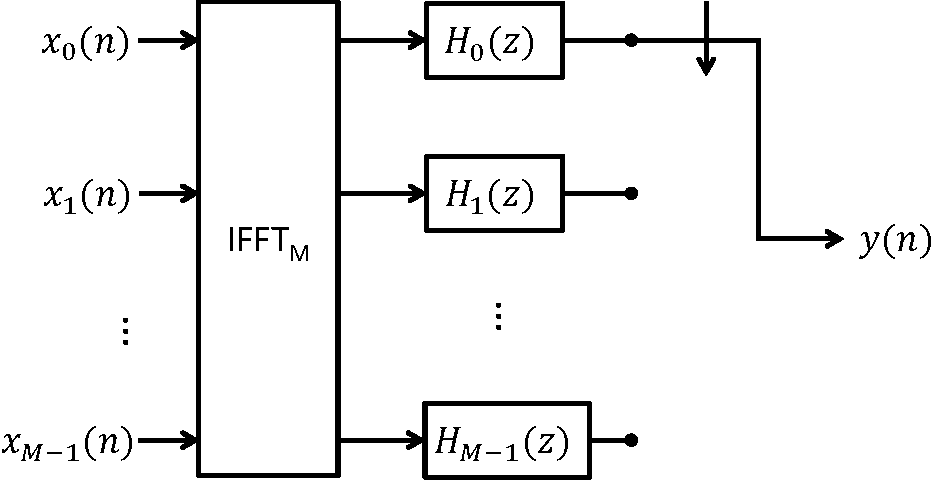
\includegraphics[height=4cm]{polyphase_synthesis}%
    \label{fig:polyphase_synthesis}}
}
\caption{Full polyphase analysis/synthesis filter bank structures}
\label{fig:poly_analysis_synthesis_structs}
\end{figure}


\subsection{Combining Analysis and Synthesis Filter Banks}
\label{sec:combine_analysis_synthesis}
The primary limitations of analysis filter banks alone are that, 1) they are
limited to a single output sample rate, and 2) they are limited to specific
channel center frequencies. These limitations are perfectly acceptable when
every signal being processed is at the same bandwidth and symbol rate, and they
are channelized with a known spacing, but in many SDR applications this is not
the case.

However, there is a clever way to continue to take advantage of these efficient
structures, while getting around the limitations: use analysis and synthesis
filter banks together. The basic idea is to completely ``deconstruct" the
spectrum with a large analysis filter bank and then allocate synthesis
filter banks for each target signal to recombine the sections of the spectrum
which contain thos signals. This approach, described by fred harris in
\cite{Harris2}, can isolate multple signal bandwidths at arbitrary center
frequencies.

Figure~\ref{fig:analysis_and_synthesis} illustrates the concept.
The first step of this process uses an analysis
filter bank to break up the wideband into small equal parts (1). Then,
synthesis filter banks are used to re-combine the parts of the signal that
correspond to signals of interest (2). Finally, complex rotators are used to
center the signal (3). 

\begin{figure}[h!]
    \begin{center}
    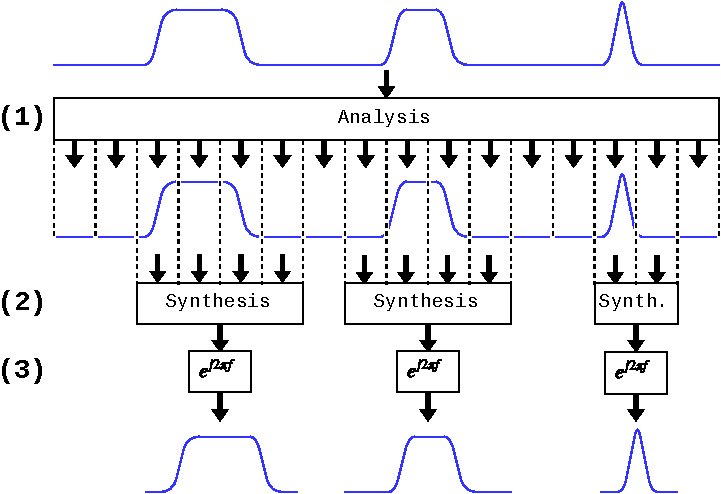
\includegraphics[width=0.8\textwidth]{polyphase}%
    \end{center}
    \caption{
Using polyphase analysis/synthesis filter bank structures in concert. Step (1)
is an analysis filter bank that breaks the signal into 16 channels, Step (2) is
a set of synthesis filter banks for each signal of interest, and Step (3) is
a complex rotators that corrects the frequency offset. Note that this figure
depicts the signal in the frequency domain, simply for ease of illustration -
all inputs and outputs are time-domain signals.
    }
    \label{fig:analysis_and_synthesis}
\end{figure}

The analysis filter bank can be running all the time, while the synthesis
filter banks and complex rotators in steps (2) and (3) can be dynamically
allocated as signals of interest are detected (by some external detector).

Unfortunately, there is an issue with this approach, as we have described it so
far. Since the analysis filter bank is maximally decimated, meaning the filter
cutoff is equal to the nyquist frequency of the output signals, the filter
rolloff aliases into the output. Then when these outputs are re-combined by 
synthesis filter banks to reconstruct a signal of interest, that aliasing is left
in the middle of the signal bandwidth.  For this reason, \cite{Harris2} utilizes
a modified version of these structures: non-maximally decimated filter banks.

\subsection{Non-Maximally Decimated Analysis/Synthesis Filter Banks}
Non-maximally decimated analysis and synthesis filter banks are much like the
analysis and synthesis filter banks we have already discussed, but modified to
use a lower decimation factor. An excellent overview of these structures can be
found in \cite{Chen1}. It starts with a general structure that can be used for
arbitrary decimation rates (where $D$ is a factor of $M$), and a realization of
this general structure when $D=M/2$.  This realization, which is used in our
simulation, can be seen in Figure~\ref{fig:poly_analysis_synthesis_nmdfb}.

\begin{figure}[h!]
\centerline{
    \subfloat[Analysis]
    {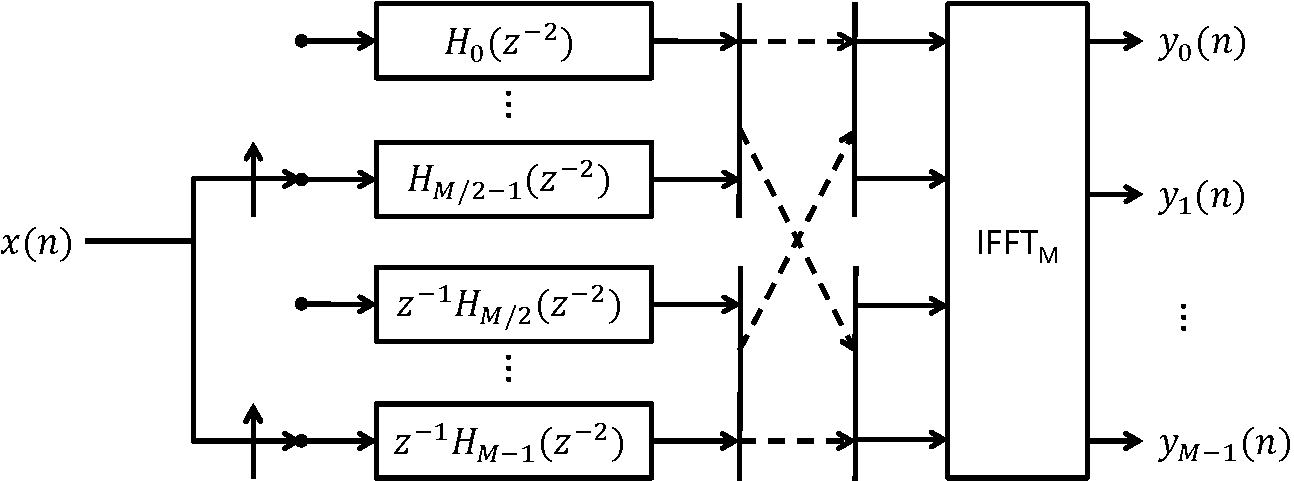
\includegraphics[height=3cm]{polyphase_analysis_nmdfb}%
    \label{fig:polyphase_analysis_nmdfb}}
    \hfill
    \subfloat[Synthesis]
    {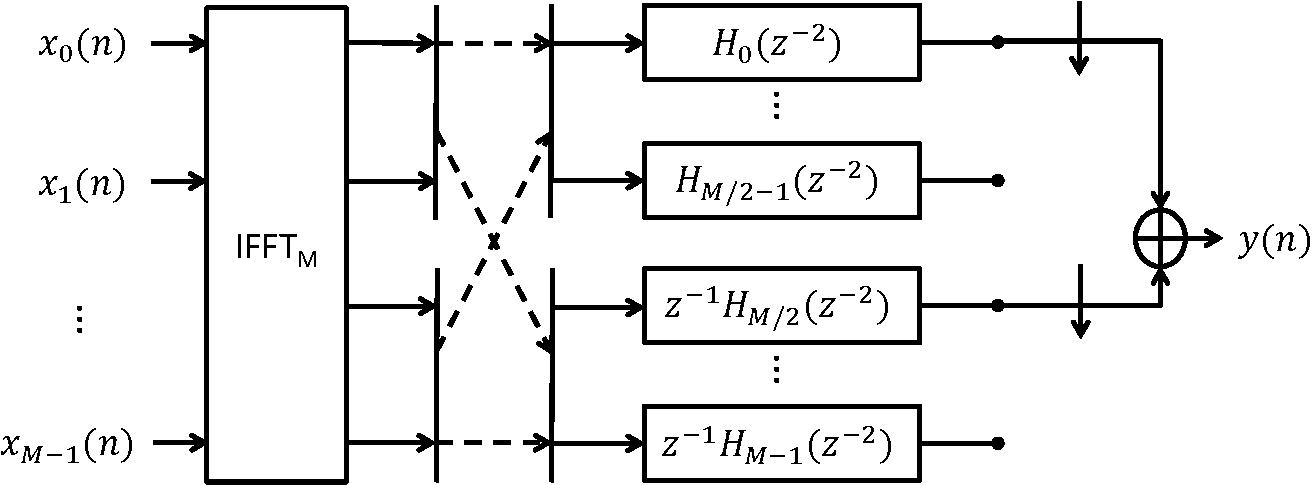
\includegraphics[height=3cm]{polyphase_synthesis_nmdfb}%
    \label{fig:polyphase_synthesis_nmdfb}}
}

\caption{Non-maximally decimated polyphase analysis/synthesis filter bank structures}
\label{fig:poly_analysis_synthesis_nmdfb}
\end{figure}

Clearly, these structures are very similar to the standard analysis and
synthesis filter banks. Let's examine the differences in the analysis filter
bank (Figure~\ref{fig:polyphase_analysis_nmdfb}), from left to right. The first
difference is that the input commutator has been replaced with a double input
commutator. This makes intuitive sense - with a double input commutator the
structure will accept half as many input samples for each output sample
compared to the standard analysis filter bank, leading to a decimation factor
of $M/2$ rather than $M$. The second difference is the filter partitions: each
partition has been downsampled by a factor of 2, and the filters on the bottom
half have been delayed by one sample.  Again, the downsampling makes intuitive
sense given the change to $D=M/2$. The next difference is the conditional
circular buffer after the filter partitions. This circular buffer simply swaps
the upper and lower halves - but it only does it for every \emph{odd} set of
samples - the even sets are simply passed through. This swapping is required to
absorb a phase offset. The final difference is the use of an M-point IFFT
rather than an FFT \cite{Chen1}.

Using these non-maximally decimated filter banks (NMDFBs) in the combined
analysis/synthesis filter bank allows the synthesis filter banks to perfectly
reconstruct the received signal.

\subsection{Limitations}
\label{sec:poly_limitations}
We have already examined the limitations of a polyphase analysis
filter bank used alone: every channel must be at the same output sample
rate, $f_s/D$, and they must have center frequencies which are multiples of
that sample rate.

If the combination analysis/synthesis structure is used then this limitation
can be avoided, however there are still other issues. First, the output sample
rate must still be a decimation of the input sample rate - arbitrary rates are
not allowed.  Also, like the overlap-save filter bank, this structure relies on
the efficiency of the FFT to save computation, and the size of the IFFT in the
analysis filter bank is directly related to the decimation factor used. If
a decimation factor with large prime factors is required then the analysis
filter bank's IFFT will be inefficient.

Finally, there is no obvious way that this structure can be efficiently
combined with SCD estimation for detection. Nothing about an polyphase filter
bank can be re-used for the detection approach discussed in this paper.


\subsection{Advantages}
\label{sec:poly_advantages}
The primary advantage of a lone polyphase analysis filter bank is its
simplicity and efficiency, but its limitations make it an untenable solution
for this project.

The combination polyphase analysis/synthesis filter bank adds some complexity,
but it is still quite efficient for the amount of flexibility that it provides.
Another major benefit of both analysis and synthesis filter banks is that they
can be implemented in hardware relatively easily. One can imagine a hardware
implementation of this structure where an analysis filter bank is always
running, and a bank of synthesis filter banks are dynamically connected and
disconnected as signals are detected.

% TODO: this needs to be expanded


\section{Simulation Results}
\label{sec:sim}
\markright{Brian H. Hulette \hfill Section \ref{sec:sim}. Simulation Results \hfill}

A MATLAB simulation of the structures described in this paper has been
created\footnote{The entire source code for this simulation is available on
Github: \url{https://github.com/TheNeuralBit/cyclo_channelizer/}}. This
simulation uses simple QPSK carriers as test signals, but the cyclostationary
detection and configurable filter bank software are applicable to many types of
signals.

\subsection{Runtime Comparison}
\label{sec:sim_runtime}

The simulation was used to compare the efficiency of the two filter bank
structures. It is important to note that, while the runtime for both structures
can clearly be improved with parallelization, this simulation is completely
single-threaded. This approach allows us to use overall runtime measurements as
an analog for the total CPU time required for each approach. Of course,
a practical implementation of either structure should run as much in parallel
as possible.

A comparison of runtimes for the overlap-save structure and the polyphase
structure can be seen in Figure~\ref{fig:block_diagram}. The plot shows the
runtime when both structures are used to simultaneously detect and tune various
numbers of signals. For each number of signals, a 10 MHz wide simulated
wideband acquisiton is created. This acquisition contains 78.125 ksymbol/s QPSK
signals distributed evenly throughout the spectrum. Each filter bank is
configured to decimate every signal down to two samples per symbol.

\begin{figure}[h!]
    \begin{center}
    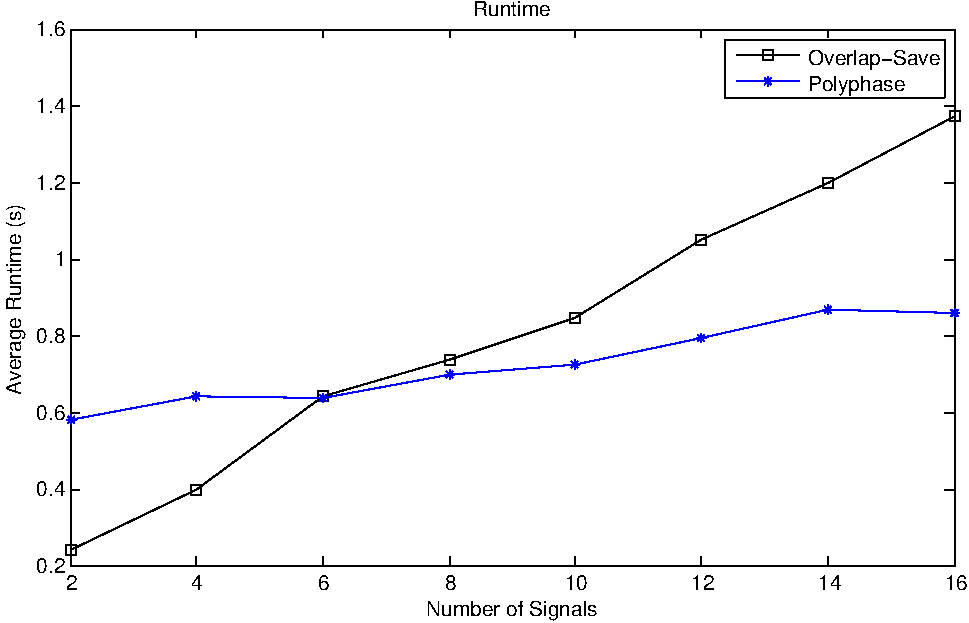
\includegraphics[width=0.7\textwidth]{runtime_comparison_250}%
    \end{center}
    \caption{Runtime comparison of detector combined with the overlap-save
             filter bank and with the polyphase analysis/synthesis filter bank}
    \label{fig:block_diagram}
\end{figure}

From this runtime comparison, we see a clear trend: for a very small number of
signals the polyphase structure is less efficient.  However, each addiditional
signal costs more time for the overlap-save filter bank to process than the
polyphase filter bank. When isolating more than six signals, the polyphase
structure is more efficient. There are two clear takeaways from this result: 1)
there is a larger cost up-front when using a polyphase filter bank, but 2) the
marginal cost for each additional signal being isolated is lower for the
polyphase filter bank. 

These takeaways are actually easy to predict just by examining the structures.
The polyphase filter bank has a large up-front cost because it must run a large
analysis channelizer no matter the number of signals being processed. In
addition, the overlap-save filter bank saves some time up-front by using
a single FFT for detection and filtering. On the other hand, for each
additional signal, the polyphase fiter bank just needs to perform one
additional small IFFT and a couple more filters at a low data rate, while the
overlap-save filter bank must perform an additional multiplication in the
frequency domain at the wideband data rate.

\begin{figure}[h!]
    \begin{center}
    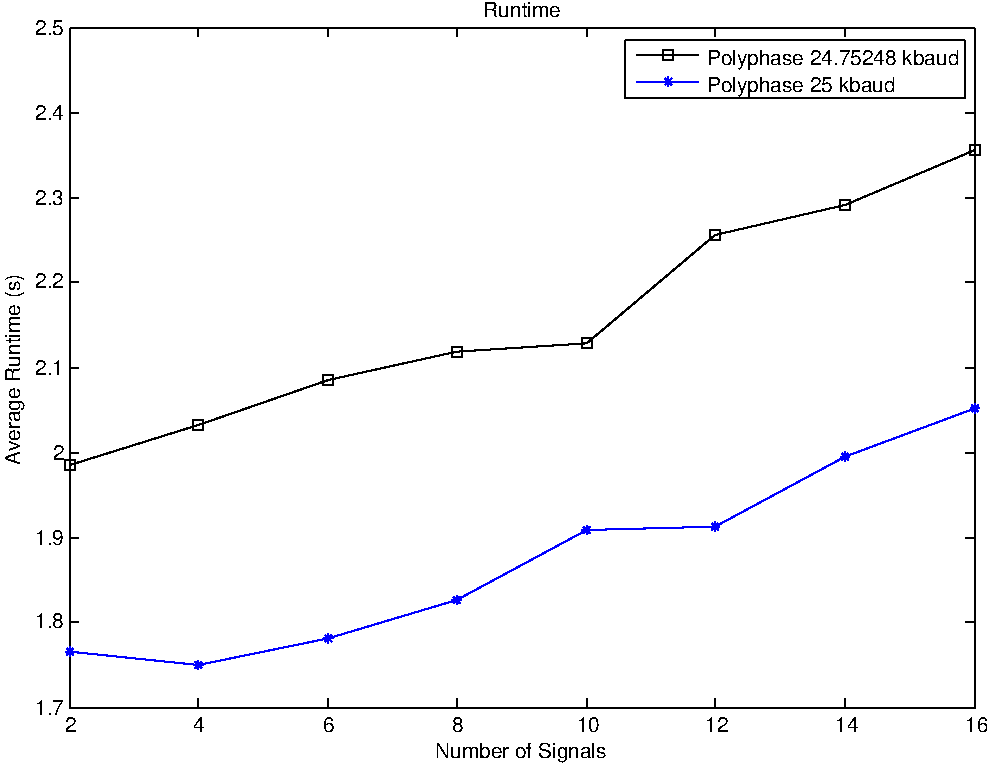
\includegraphics[width=0.7\textwidth]{fft_runtime_comparison}%
    \end{center}
    \caption{Runtime comparison of detector combined with the polyphase filter
             bank. The 24.75248 kbaud signal requires a 202 point IFFT, while the 25
             kbaud signal can use a 200 point IFFT. The former has a large prime factor,
             101, leading to a much longer runtime. A similar effect can be seen in the
             overlap-save structure.}
    \label{fig:block_diagram}
\end{figure}

The situation simulated in this scenario represents a best-case scenario for
both structures. The baud rate of the test signals was chosen so that the
decimation factor would be a power of two. This means that polyphase analysis
filter bank and the large FFT in the overlap-save filter bank can use a very
efficient power of two FFT size. Figure~\ref{fig:block_diagram} illustrates the
effect of a poor decimation factor on the polyphase filter bank - just changing
the decimation factor from 200 to 202 severely harms performance. It should be
noted that, in general, it is easy to avoid this pitfall for both structures by
decimating with a good FFT size. If a different narrowband sample rate is
required, the outputs can be resampled after the filter bank.

In both of these test cases, since all of the signals are the same bandwidth,
the polyphase filter bank can be designed so that only size $M=2$ synthesis
filter banks are required.  One can imagine a worst-case scenario for the
polyphase filter bank where there is one low bandwidth signal and many high
bandwidth signals.  In this scenario, a large analysis filter bank is required
to isolate the low bandwidth signal, but then very large synthesis filter banks
must be used to reconstruct each of the high bandwidth signals.

Clearly, it is difficult to say definitively that either structure is much more
efficient than the other. For any given application, each structure should be
evaluated to determine which is better suited for it.


\section{Conclusion}
\label{sec:conclusion}
\markright{Brian H. Hulette \hfill Section \ref{sec:conclusion}. Conclusion \hfill}
Simulations of a cyclostationary detector and two separate configurable filter
bank structures, an overlap-save filter bank and a combination polyphase
analysis/synthesis filter bank, have been presented. Both filter bank
structures were combined with the cyclostationary detector in order to evaluate
their performance when detecting and isolating QPSK signals at various symbol
rates in various wideband test signals. Both structures proved effective at accurately
detecting and isolating these signals, but the runtime performance of each
varied greatly depending on the number of signals being isolated. In general,
the overlap-save filter bank is a better choice for a smaller number of signals,
and the polyphase filter bank is better for a large number of signals.

Currently these simulations only uses the beginning of the test signal for
detection, but in an actual implementation the detector would be running
continuously and dynamically directing the filter banks to begin processing new
signals. It should be noted that in this described system, both filter banks would
need to have knowledge of the required signal bandwidths and output sample
rates before processing begins, so that appropriate filters can be designed, and
in the case of the polyphase analysis/synthesis filter bank, so that the size
of the analysis filter bank can be chosen.

\subsection{Future Work}
This work could be extended in many different ways. In this project, the
limitations of the various structures were taken as a given, however many of
these limitations can actually be avoided. For example, Harris shows that it is
in fact possible to adjust the output sample rate of the analysis filter bank
by adjusting the input commutator \cite{Harris1}. That topic was left out of this
simulation since it is difficult to devise a flexible version of it that will
work for any sample rate. Future work could focus on what output sample rates
are possible and devise an approach for a general purpose solution.

% - using single FFT to estimate cyclic spectra for non-perfect cyclic frequencies
Another limitation taken as a given is that SCD estimation with a single FFT is
impossible for cyclic frequencies that do not satisfy
Equation~\ref{eq:cyclo_freqs} - but this could potentially be overcome as well.
For cyclic frequencies, where $\alpha/2$ does not correspond to a specific FFT
bin the FFT could be interpolated before shifting. This would not be perfectly
accurate, but it would be worth evaluating how close of an approximation this
yields. Additionally, one could evaluate how complex of an interpolation could
be used while still maintaining the computational advantage of using a single FFT.

% - Evaluate Pd vs. Pfa
% - Low SNR
%The only presented test case was very low noise - it would be beneficial to
%evaluate how well the detector and channelizers work as a function of noise
%power. A Monte Carlo test could be performed to evaluate the detector's
%probability of detection, $P_d$, vs. noise power at a given threshold. Both
%channelizers should also be evaluated by plotting the Bit Error Rate (BER) of
%every output channel as a function of noise power. Perhaps we will find that
%one of the channelizers harms the signal integrity.

% - comparison of computational complexity
Finally, it would be useful to complement the simulated runtime analysis with
an in-depth theoretical analysis of the computational complexity of both
combined detector/filter banks. 

% - Filter Design (TODO)

%%%%%%%%%%%%%%%%%
%
% Include an EPS figure with this command:
%   \epsffile{filename.eps}
%

%%%%%%%%%%%%%%%%
%
% Do tables like this:

% \begin{table}
% \caption{The Graduate School wants captions above the tables.}
%\begin{center}
% \begin{tabular}{ccc}
% x & 1 & 2 \\ \hline
% 1 & 1 & 2 \\
% 2 & 2 & 4 \\ \hline
% \end{tabular}
%\end{center}
% \end{table}

%%%%%%%%%%%%%%%%%%%%%%%%%%%%%%%%

% If you are using BibTeX, uncomment the following:
\nocite{*}
\bibliographystyle{IEEEtran}
\bibliography{bibliography}
%
% Otherwise, uncomment the following:
% \chapter*{Bibliography}

% \appendix

\end{document}
